\begin{figure*}[t]
  \centering
\begin{subfigure}[t]{0.35\linewidth}

\includegraphics[width=\linewidth]{figures/optimal_sd/oracle/legend_only.pdf}
\end{subfigure}

\begin{subfigure}[b]{0.22\linewidth}
    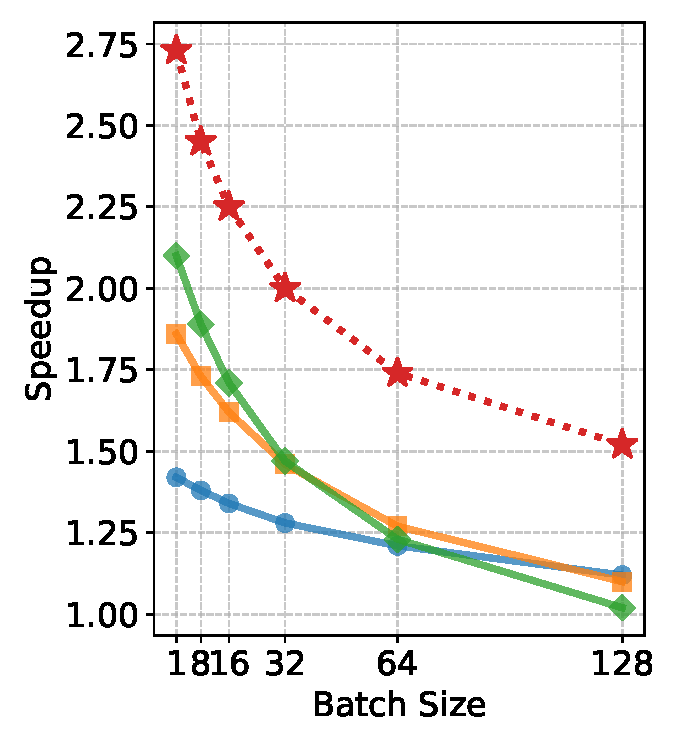
\includegraphics[width=\linewidth]{figures/optimal_sd/oracle/ngram_instructcoder_speedup.pdf}
    \caption{$n$-gram, InstructCoder.}
    \label{fig:speedup-oracle-ngram-instructcoder}
\end{subfigure}
\begin{subfigure}[b]{0.22\linewidth}
    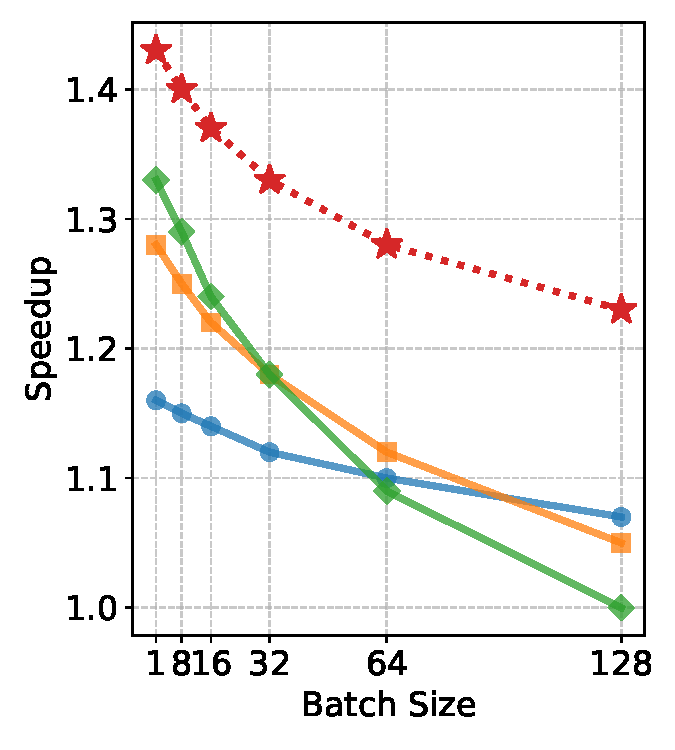
\includegraphics[width=\linewidth]{figures/optimal_sd/oracle/ngram_sharegpt_speedup.pdf}
    \caption{$n$-gram, ShareGPT.}
    \label{fig:speedup-oracle-ngram-sharegpt}
\end{subfigure}
\begin{subfigure}[b]{0.22\linewidth}
    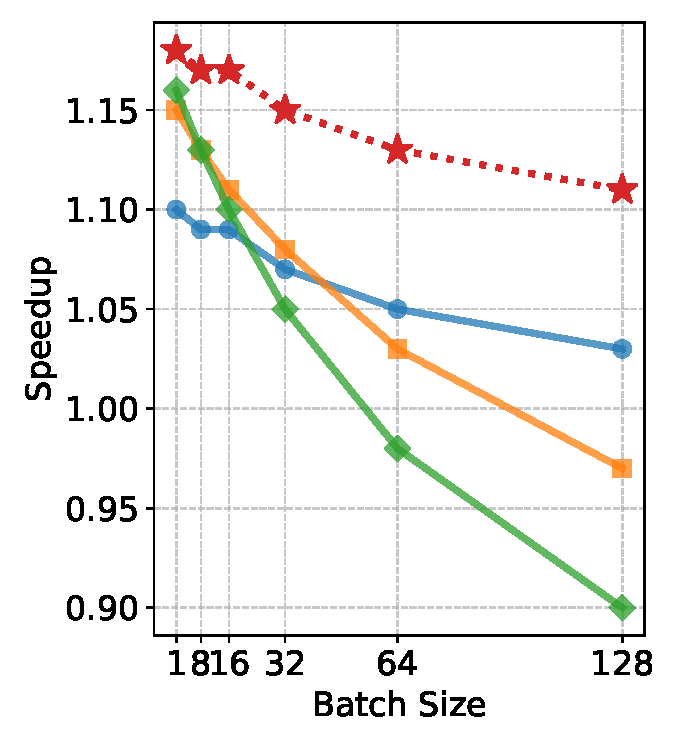
\includegraphics[width=\linewidth]{figures/optimal_sd/oracle/ngram_gsm8k_speedup.pdf}
    \caption{$n$-gram, GSM8K.}
    \label{fig:speedup-oracle-ngram-gsm8k}
\end{subfigure}
\begin{subfigure}[b]{0.22\linewidth}
    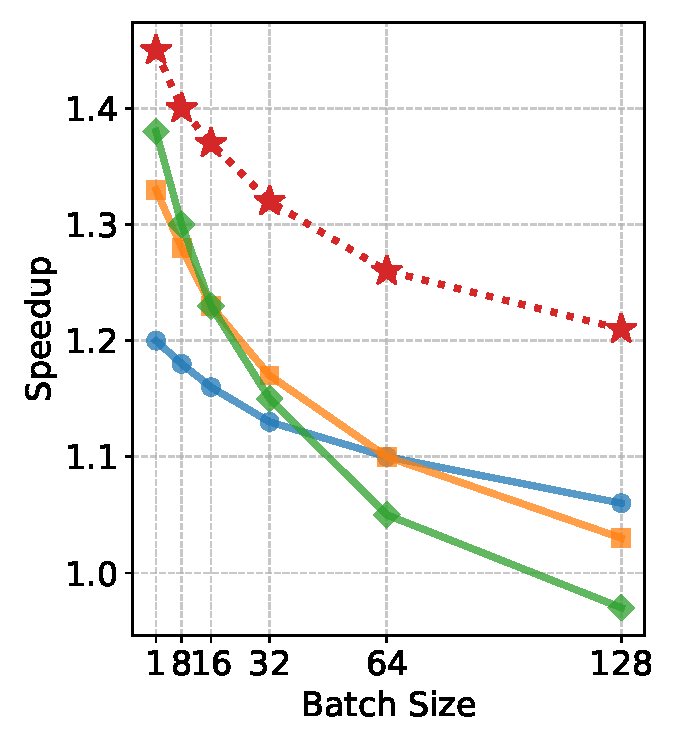
\includegraphics[width=\linewidth]{figures/optimal_sd/oracle/ngram_cnn_speedup.pdf}
    \caption{$n$-gram, CNN/DailyMail.}
    \label{fig:speedup-oracle-ngram-cnn}
\end{subfigure}

\begin{subfigure}[b]{0.22\linewidth}
    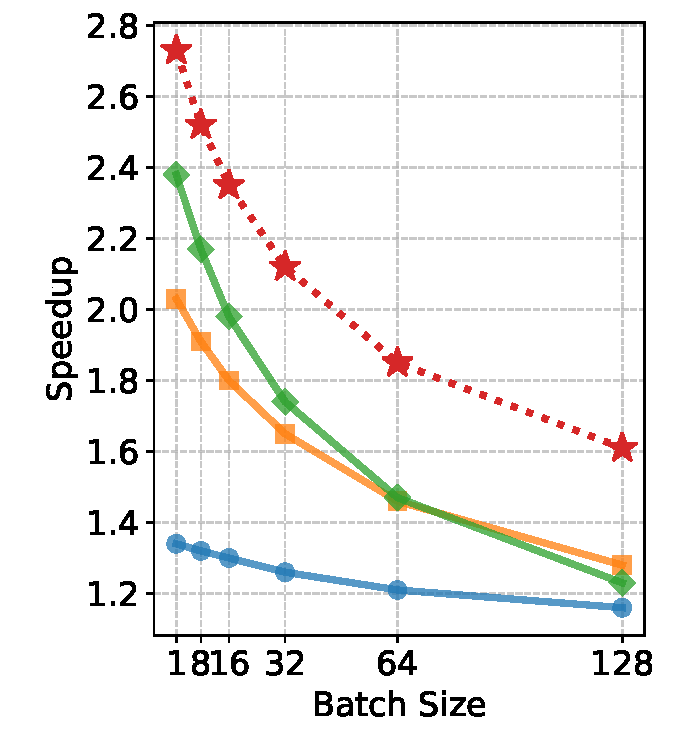
\includegraphics[width=\linewidth]{figures/optimal_sd/oracle/eagle_instructcoder_speedup.pdf}
    \caption{EAGLE, InstructCoder.}
    \label{fig:speedup-oracle-eagle-instructcoder}
\end{subfigure}
\begin{subfigure}[b]{0.22\linewidth}
    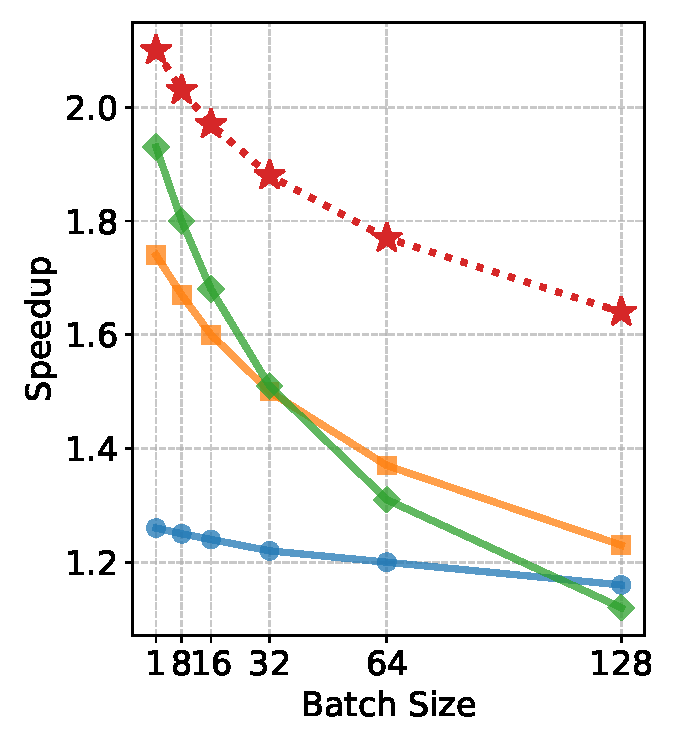
\includegraphics[width=\linewidth]{figures/optimal_sd/oracle/eagle_sharegpt_speedup.pdf}
    \caption{EAGLE, ShareGPT.}
    \label{fig:speedup-oracle-eagle-sharegpt}
\end{subfigure}
\begin{subfigure}[b]{0.22\linewidth}
    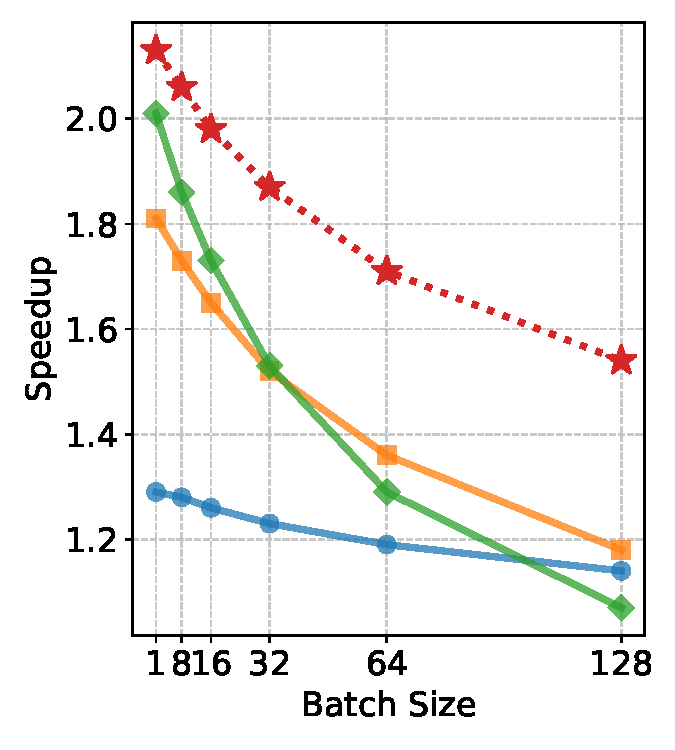
\includegraphics[width=\linewidth]{figures/optimal_sd/oracle/eagle_gsm8k_speedup.pdf}
    \caption{EAGLE, GSM8K.}
    \label{fig:speedup-oracle-eagle-gsm8k}
\end{subfigure}
\begin{subfigure}[b]{0.22\linewidth}
    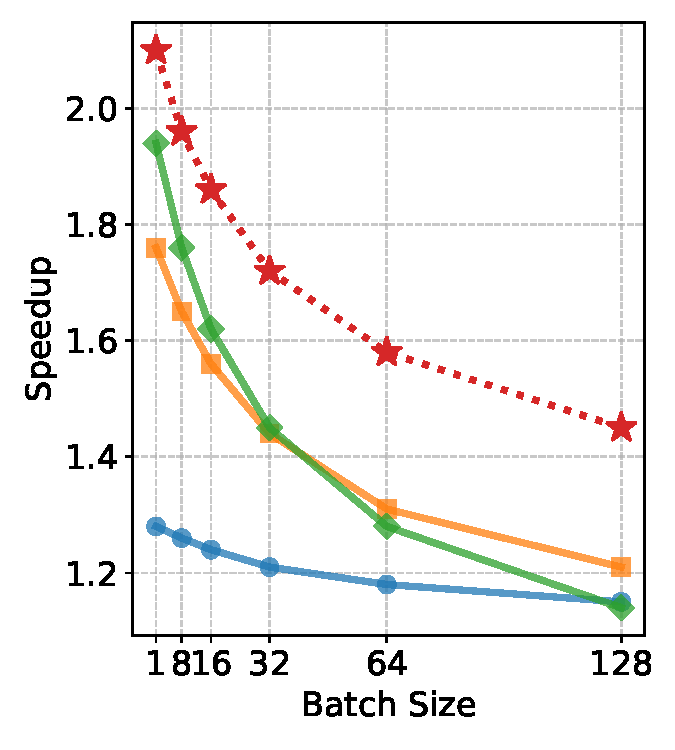
\includegraphics[width=\linewidth]{figures/optimal_sd/oracle/eagle_cnn_speedup.pdf}
    \caption{EAGLE, CNN/DailyMail.}
    \label{fig:speedup-oracle-eagle-cnn}
\end{subfigure}
    
    % \vspace{-0.2in}
    \caption{Oracle vs fixed proposed length speedup on Llama3.1-8B.}
    \label{fig:speedup-oracle}
    % \vspace{-0.1in}
%
\end{figure*}


\begin{figure*}[h]
  \centering
      \begin{subfigure}[b]{0.24\linewidth}
    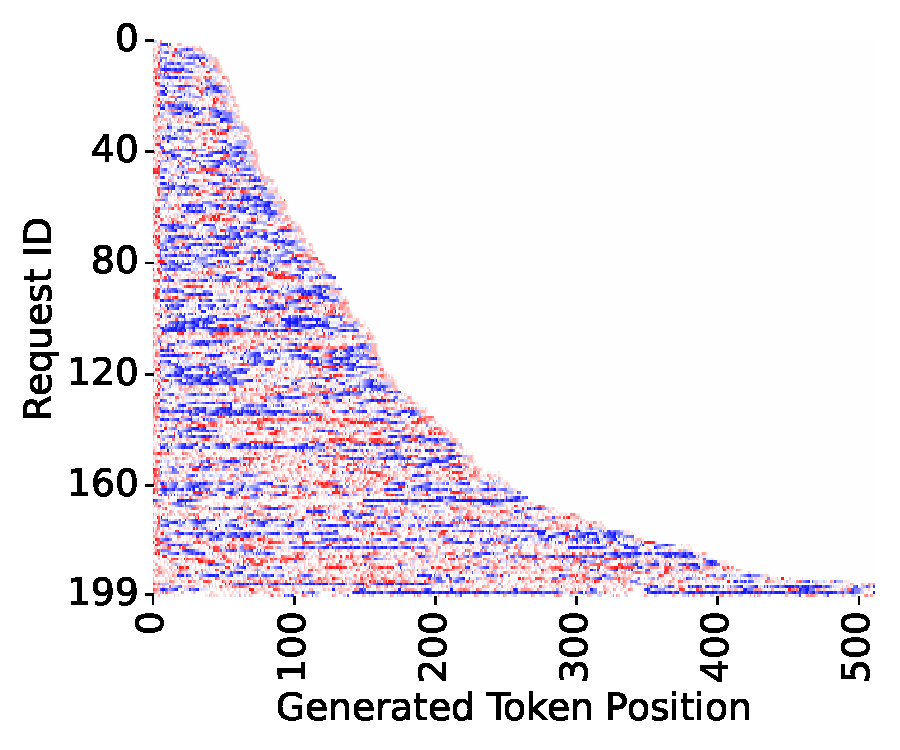
\includegraphics[width=\linewidth]{figures/optimal_sd/diff/diff_eagle3_ngram_instructcoder_acceptance_stats.pdf}
    \caption{InstructCoder}
    \label{fig:acc-diff-instrcutcoder}
  \end{subfigure}
      \begin{subfigure}[b]{0.24\linewidth}
    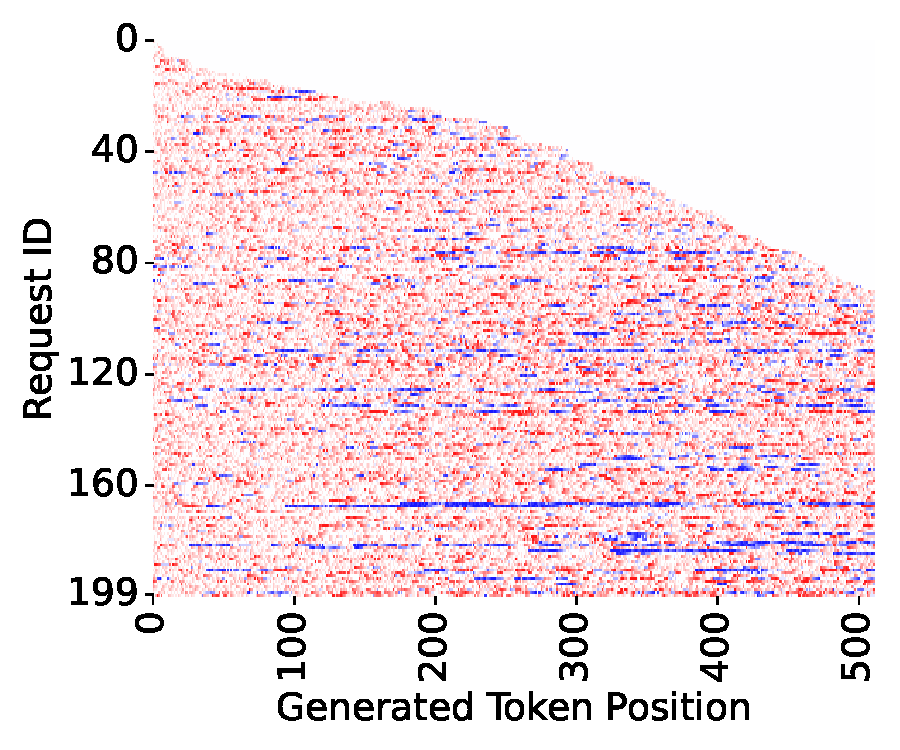
\includegraphics[width=\linewidth]{figures/optimal_sd/diff/diff_eagle3_ngram_sharegpt_acceptance_stats.pdf}
    \caption{ShareGPT}
    \label{fig:acc-diff-sharegpt}
  \end{subfigure}
      \begin{subfigure}[b]{0.24\linewidth}
    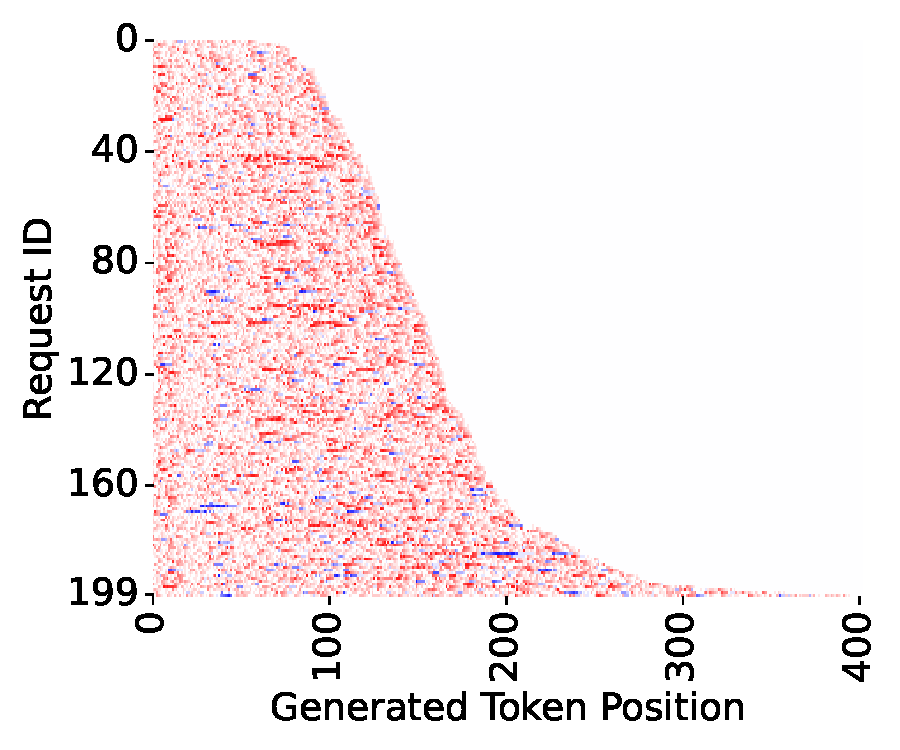
\includegraphics[width=\linewidth]{figures/optimal_sd/diff/diff_eagle3_ngram_gsm8k_acceptance_stats.pdf}
    \caption{GSM8K}
    \label{fig:acc-diff-gsm8k}
  \end{subfigure}
          \begin{subfigure}[b]{0.24\linewidth}
    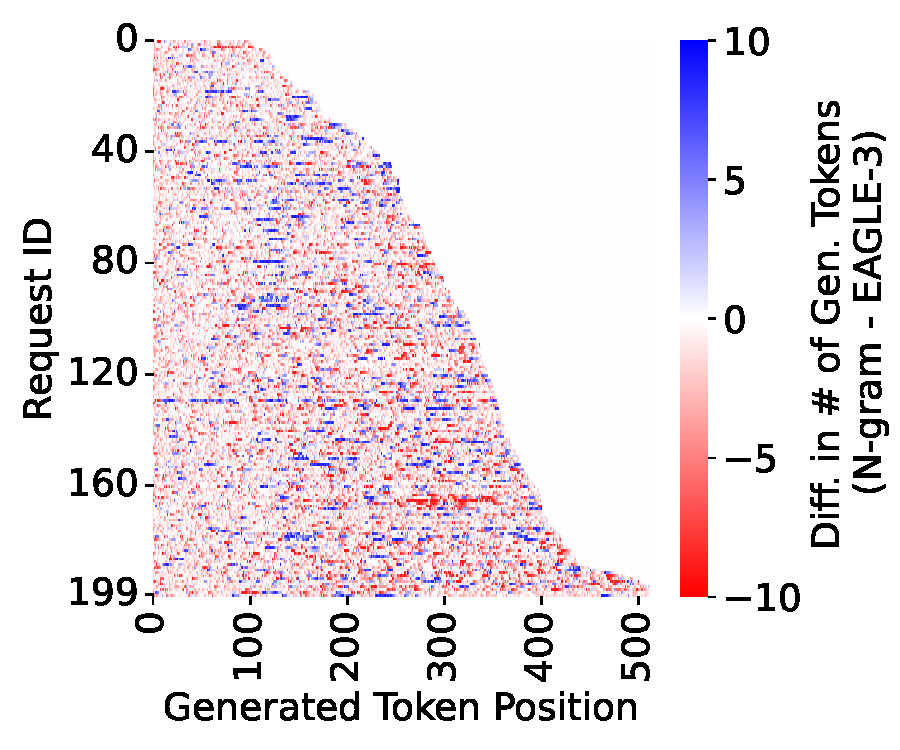
\includegraphics[width=\linewidth]{figures/optimal_sd/diff/diff_eagle3_ngram_cnn_acceptance_stats.pdf}
    \caption{CNN/DailyMail}
    \label{fig:acc-diff-cnn}
  \end{subfigure}
  \caption{Per-position accepted-length difference between $n$-gram and EAGLE on Llama 3.1-8B. Red indicates positions where EAGLE accepts longer spans, while blue indicates positions favoring $n$-gram. The figure illustrates that different speculative decoding methods exhibit distinct acceptance behaviors across decoding positions.}
\label{fig:acc-diff}
\end{figure*}


\begin{figure*}
\centering
\begin{subfigure}[t]{0.65\linewidth}
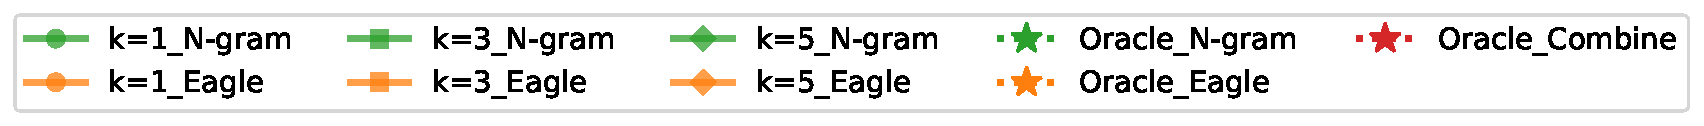
\includegraphics[width=\linewidth]{figures/optimal_sd/oracle/combined_legend_only.pdf}
\end{subfigure}

    \begin{subfigure}[b]{0.22\linewidth}
      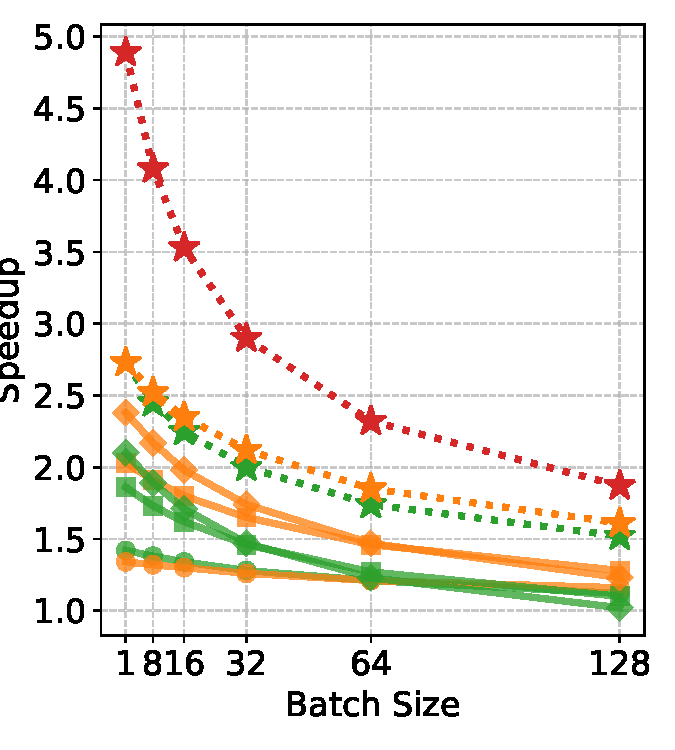
\includegraphics[width=\linewidth]{figures/optimal_sd/oracle/combined_instructcoder_speedup.pdf}
      \caption{InstructCoder}
      \label{fig:opt-speedup-instrcutcoder}
  \end{subfigure}
  \begin{subfigure}[b]{0.22\linewidth}
      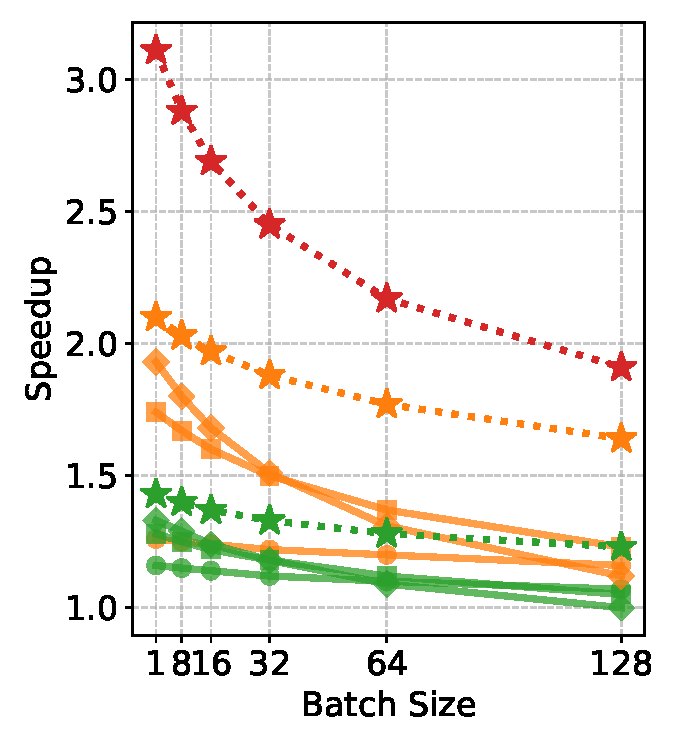
\includegraphics[width=\linewidth]{figures/optimal_sd/oracle/combined_sharegpt_speedup.pdf}
      \caption{ShareGPT}
      \label{fig:opt-speedup-sharegpt}
  \end{subfigure}
   \begin{subfigure}[b]{0.22\linewidth}
      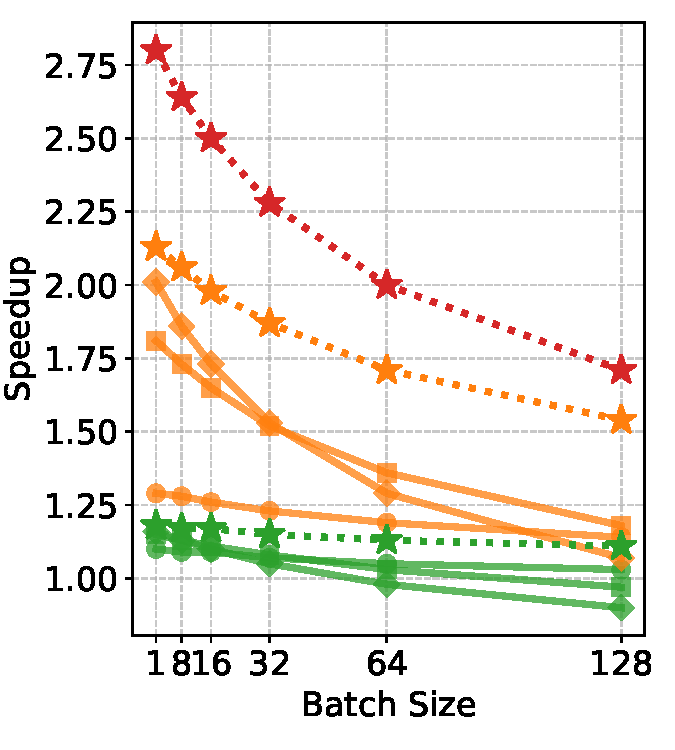
\includegraphics[width=\linewidth]{figures/optimal_sd/oracle/combined_gsm8k_speedup.pdf}
      \caption{GSM8K}
      \label{fig:opt-speedup-gsm8k}
  \end{subfigure}
      \begin{subfigure}[b]{0.22\linewidth}
      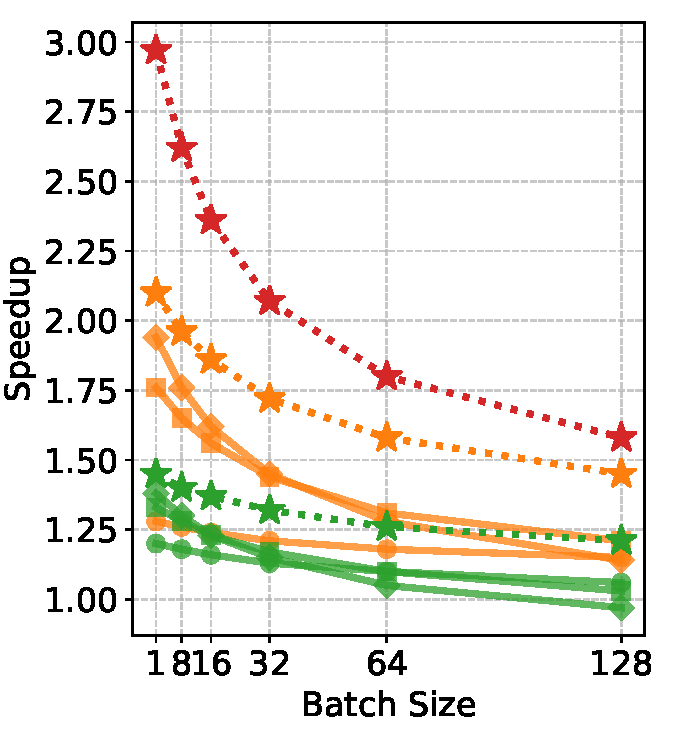
\includegraphics[width=\linewidth]{figures/optimal_sd/oracle/combined_cnn_speedup.pdf}
      \caption{CNN/DailyMail}
      \label{fig:opt-speedup-cnn}
  \end{subfigure}
  \caption{Combining different SD methods for optimal speedup on Llama3.1-8B.}
  \label{fig:opt-speedup}
\end{figure*}



\section{Theoretical Speedup Upper Bound of Speculative Decoding}
\label{sec:theoretical-speedup}
% With the understanding of acceptance behavior, we can now estimate the potential speedup if we could perfectly predict the number of accepted tokens at each position. To estimate zero-waste speculative decoding, we proposed generating a very long speculative sequence—for example, 20 tokens at each position—to observe how many tokens could be accepted at each step. After each generation step, even if multiple tokens were accepted, we discarded all but one and advanced to the next position. Essentially, we recorded the maximum number of tokens that could be accepted at each speculative decoding step. Using this information, along with the execution time breakdown from the previous section, we can estimate the potential speedup if we knew the exact number of accepted tokens at each position in advance.
In this section, we aim to derive an upper bound of the speedup achievable by SD. Our goal is to understand how far current SD methods are from the theoretical optimum, assess their current performance limits, and highlight potential directions for future research.

As discussed in \autoref{sec:breakdown}, verification time dominates the overall execution cost. This naturally raises the question: \emph{if we could eliminate wasted verification by avoiding the verification of tokens that would ultimately be rejected, what is the maximum speedup that speculative decoding could achieve?
In other words, assuming an oracle—or a sufficiently accurate mechanism—that proposes only tokens likely to be accepted, what is the upper bound on the achievable speedup?} In the following section, we try to derive this number and understand the gap between current speedup and theoritical upper bound.

Moreover, as observed in \autoref{sec:acc-behavior}, different SD variants exhibit distinct acceptance behaviors. Specifically, they differ in the number of tokens accepted at each generation step. To better understand the true performance upper bound, we investigate whether combining different SD strategies could yield an even more optimal acceptance pattern and, consequently, higher overall efficiency. 

%therefore conclude with a list of open challenges for future work inspired by our study.



\subsection{Minimal Verification Cost}
We begin by addressing the following question: if we could minimize the verification cost, what is the maximum speedup that speculative decoding could achieve? To explore this, we compare the performance of using a fixed proposed length against that of an oracle-based proposed length. The oracle setup assumes that the number of tokens accepted at each generation step is known in advance. At each step, we set the proposed length equal to the actual accepted length, ensuring that all proposed tokens are accepted. This setup effectively simulates the ideal case where verification incurs no rejection overhead.

One might argue that if all proposed tokens can be perfectly accepted, the large model would no longer be necessary. While that is theoretically correct, it is practically unattainable—no proposal mechanism can perfectly predict future target tokens. Hence, the oracle configuration serves purely as an upper bound on the achievable speedup of speculative decoding, highlighting the performance ceiling that real methods can approximate.

We conduct this analysis using Llama 3.1-8B on the InstructorCoder, ShareGPT, GSM8K, and CNN/DailyMail datasets. We observe a substantial gap between the oracle speedup and the speedup achieved with a fixed proposal length. The oracle speedup represents an upper bound in which the accepted length at each decoding step is known in advance, and the system proposes exactly that many tokens. As a result, every proposed token is accepted, eliminating any wasted speculation.

 As shown in \autoref{fig:speedup-oracle}, on the Instructcoder dataset with a batch size of one and $n$-gram as the SD method, the oracle setup achieves a speedup of approximately 2.75$\times$, whereas the fixed proposed length configuration attains about 2.1$\times$ for the best proposed length of 5. Moreover, the gap generally widens as batch size increases: the fixed-$k$ curves drop much faster, while the oracle speedup degrades more gently. This trend is consistent with our observation in \autoref{fig:exec-breakdown}. As batch size grows, verification takes up a larger share of the decoding time, so fixed-$k$ methods would incur larger overhead for verifying draft tokens that are ultimately rejected.

% An interesting pattern emerges when comparing $n$-gram and EAGLE. With small batch sizes, the gap between oracle and fixed-length speedups is noticeably smaller on ShareGPT. As discussed in \autoref{sec:acc-behavior}, when $n$-gram successfully identifies a match, it tends to be correct, leading to a higher acceptance rate—that is, fewer rejected tokens and reduced verification overhead. Consequently, there is less room for further reducing verification cost. However, as the batch size increases, the system becomes increasingly compute-bound, causing the performance gap to widen for both methods.



% \begin{figure}[t]
%   \centering
%   \begin{subfigure}[b]{0.45\linewidth}
%     \includegraphics[width=\linewidth]{figures/optimal_sd/oracle/eagle3_instructcoder_speedup.pdf}
%     \caption{Instructcoder, Eagle}
%   \end{subfigure}
%   \begin{subfigure}[b]{0.45\linewidth}
%     \includegraphics[width=\linewidth]{figures/optimal_sd/oracle/eagle3_sharegpt_speedup.pdf}
%     \caption{ShareGPT, Eagle}
%   \end{subfigure}
%   \caption{Oracle, preliminary predictor, and fixed proposed length speedup for Eagle.}
%   \label{fig:speedup-oracle-eagle}
% \end{figure}

% \textbf{Heuristic-based Accepted Length Predictor.} While previous work~\cite{agrawal2024adaedl, zhang2025draftmodelknowsstop} explores different means to reduce verification cost, we instead aim to understand how the current optimization methods compare to the theoretical upper bound and whether simple heuristics can help close this gap.
% We experiment with a lightweight predictor that leverages the draft method’s confidence to decide whether to send proposed tokens for verification. In SD, after the draft method generates a sequence of candidate tokens, only those with confidence above a threshold (e.g., 0.3 or 0.7) are forwarded for verification, while low-confidence tokens are skipped. The detailed algorithm is described in Appendix~\ref{appendix:predictor}.
% As shown by the purple lines in \jerry{todo}, the confidence-based predictor yields modest improvements in the speedup and narrows the gap toward the oracle performance. However, the remaining gap is still substantial. The predictor must be both lightweight—since it lies on the critical path—and sufficiently accurate to effectively reduce unnecessary verification of rejected tokens. We believe this direction holds great potential for further improving the efficiency of speculative decoding.


\subsection{An Adaptive Approach to Achieve Optimal Speedup}
Although EAGLE generally outperforms the $n$-gram method, 
% —for example, on the ShareGPT dataset, the oracle speedup of $n$-gram peaks at only about 1.2$\times$, which remains below EAGLE’s performance—
a closer inspection of acceptance behavior reveals complementary strengths between the two. 
As illustrated in \autoref{fig:acc-diff}, the per-position differences in accepted tokens exhibit alternating regions of red (favoring EAGLE) and blue (favoring $n$-gram), indicating that the two methods excel under different conditions. This behavior is intuitive: for example, in code snippets with strong local regularities or recurring grammatical patterns, $n$-gram can often find exact matches, which are likely to be correct.
In such cases, because $n$-gram incurs substantially lower proposing overhead, it can be the more efficient choice. At other positions where local repetition is weaker, EAGLE serves as a robust fallback, since it proposes correct tokens across diverse contexts more consistently.



This naturally brings up the next question: \emph{can we combine their advantages to achieve even higher overall speedups?}

To explore the upper bound on achievable speedup, we assume a \emph{perfect} predictor that can (1) determine which method performs best at each position, and (2) accurately predict the number of tokens that will be accepted at that position. Under this idealized assumption, we measure the maximum possible speedup attainable by speculative decoding.

It is important to note the simplifications in this setup, which represent an upper bound on achievable performance. First, we assume the predictor is flawless in determining the better method for each position. Second, we presume perfect knowledge of the number of tokens each method can accept at every position. 
% Third, we simplify the overhead comparison by using $n$-gram's proposing overhead, which is generally lower than Eagle's. This choice allows us to estimate the best-case scenario. 
Finally, we do not account for the overhead of maintaining the KV cache for EAGLE's proposing head, which would otherwise require partial prefills if a request was paused and resumed.


Under these assumptions, we report the best achievable speedup in \autoref{fig:opt-speedup}. \textbf{Oracle\_Combine} represents a theoretical upper bound in which, at each generation position, the method (EAGLE or $n$-gram) that yields the longer accepted span is selected. The resulting accepted length is then used as the proposed length. Compared to the best fixed strategy, \textbf{Oracle\_Combine} exposes substantial additional headroom, achieving up to a $2.2\times$ further speedup.

The size of this headroom depends strongly on the workload. InstructCoder shows the largest gap between existing methods and Oracle\_Combine, matching \autoref{fig:acc-diff} where red and blue regions alternate frequently, i.e., there are many positions where one method clearly outperforms the other. ShareGPT and CNN/DailyMail exhibit similar but smaller gains, indicating more limited but still meaningful room for the methods to complement each other. In contrast, GSM8K offers little additional benefit from combining because $n$-gram rarely achieves long acceptances, so \textbf{Oracle\_Combine} stays close to \textbf{Oracle\_Eagle}. 

Taken together, these results point to a promising direction for future work: developing an accurate yet lightweight predictor capable of adapting to varying levels of acceptance behavior across workloads, requests and token positions.

% Let the figures stay with this section, instead of overflowing to the reference page.
% \clearpage

% With these assumptions, we present the optimal speedup by combining the two methods in \autoref{fig:opt-speedup}. Specifically, \textbf{Oracle\_Combine} represents the theoretical upper bound obtained by selecting, at each position, the SD variant (EAGLE or $n$-gram) that yields the longer accepted sequence. 
% We observe a substantial gap between the current methods and oracle speedups, reaching over 3$\times$ improvement when the batch size is below 32. This indicates a promising direction for future work, though it poses challenges such as developing an accurate yet lightweight predictor capable of adapting to varying levels of acceptance behavior variance.

% \begin{figure}[h]
%   \centering
%   \begin{subfigure}[b]{0.35\linewidth}
%     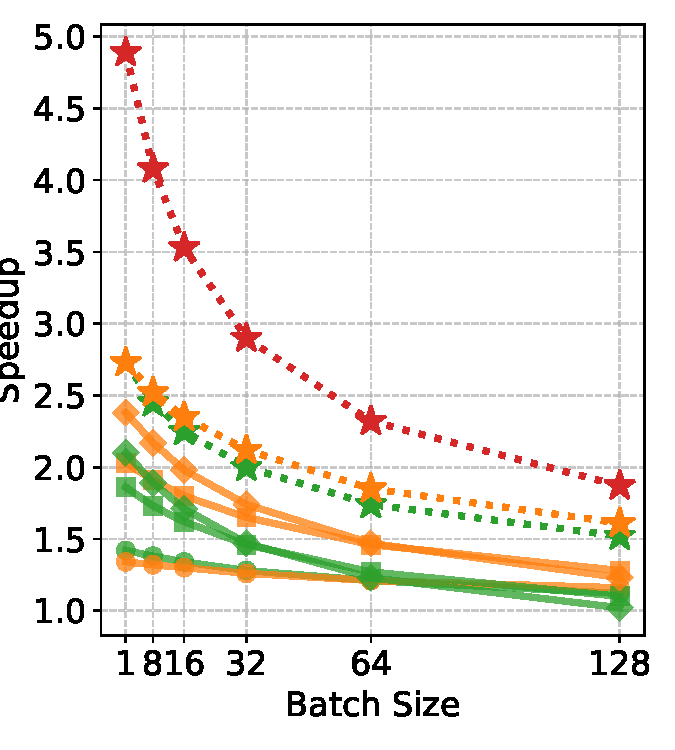
\includegraphics[width=\linewidth]{figures/optimal_sd/oracle/combined_instructcoder_speedup.pdf}
%     \caption{InstructCoder}
%   \end{subfigure}
%   \begin{subfigure}[b]{0.6\linewidth}
%     \includegraphics[width=\linewidth]{figures/optimal_sd/oracle/singlepage_plot_plus_legend.pdf}
%     \caption{ShareGPT}
%    \end{subfigure}
%   \caption{Oracle combined speedup.}
%   \label{fig:acc-combine}
% \end{figure}